\documentclass{mwrep}

% Polskie znaki
\usepackage{polski}
\usepackage[utf8]{inputenc}
\usepackage[T1]{fontenc}
\usepackage{lmodern}
\usepackage{indentfirst}

% Strona tytułowa
\usepackage{pgfplots}
\usepackage{siunitx}
\usepackage{paracol}

% Pływające obrazki
\usepackage{float}
\usepackage{svg}
\usepackage{graphicx}

% table of contents refs
\usepackage{hyperref}
\usepackage{cleveref}
\usepackage{booktabs}
\usepackage{listings}
\usepackage{hyperref}


\SendSettingsToPgf
\title{\bf Zarządzanie pamięcią \\ Raport \vskip 0.1cm}
\author{Jakub Sikora}
\date{\today}
\pgfplotsset{compat=1.15}	
\begin{document}

\makeatletter
\renewcommand{\maketitle}{\begin{titlepage}
		\begin{center}{
				\LARGE {\bf Politechnika Warszawska}}\\
			\vspace{0.4cm}
			{\LARGE {\bf Wydział Elektroniki i Technik Informacyjnych}}\\
			\vspace{5cm}
			{\bf \LARGE \mbox{Systemy operacyjne} \vskip 0.1cm}
		\end{center}
		\vspace{0.1cm}

		\begin{center}
			{\bf \LARGE \@title}
		\end{center}

		\vspace{10cm}
		\begin{paracol}{2}
			\addtocontents{toc}{\protect\setcounter{tocdepth}{1}}
			\subsection*{Zdający:}
			\bf{ \Large{ \noindent\@author \par}}
			\addtocontents{toc}{\protect\setcounter{tocdepth}{2}}

			\switchcolumn \addtocontents{toc}{\protect\setcounter{tocdepth}{1}}
			\subsection*{Prowadzący:}
			\bf{\Large{\noindent mgr. inż. Aleksander \\ Pruszkowski}}
			\addtocontents{toc}{\protect\setcounter{tocdepth}{2}}

		\end{paracol}
		\vspace*{\stretch{6}}
		\begin{center}
			\bf{\large{Warszawa, \@date\vskip 0.1cm}}
		\end{center}
	\end{titlepage}
}
\makeatother
\maketitle

\tableofcontents

\chapter{Treść zadania}
\label{TRESC}

\section{Cel zadania}
\label{TRESC::CEL}
Domyślnie w systemie Minix algorytmem wyboru wolnego bloku z listy
wolnych bloków, wykorzystywanym do realizacji funkcji systemowych FORK i
EXEC, jest algorytm first fit, czyli wybierany jest pierwszy blok
pamięci o wystarczającym rozmiarze z listy bloków wolnych.

Celem ćwiczenia jest zmiana domyślnego algorytmu przydziału pamięci w
systemie Minix. Należy umożliwić wybór algorytmu wyboru bloku z listy
bloków wolnych między standardowym first fit a tzw. algorytmem worst
fit, czyli takim, w którym wybierany jest blok pamięci z listy wolnych
bloków o największym rozmiarze.
\section{Zadanie do zrealizowania}
\label{TRESC::ZADANIE}
Należy zdefiniować dwie dodatkowe funkcje systemowe, identyfikowane stałymi
HOLE\_{}MAP oraz WORST\_{}FIT.

\subsection{HOLE\_{}MAP}
\label{TRESC::ZADANIE::HOLEMAP}
Funkcja systemowa HOLE\_{}MAP powinna umożliwiać zdefiniowanie własnej
funkcji o sygnaturze:

\begin{lstlisting}
    int hole_map(void *buffer, size_t nbytes)  
\end{lstlisting}

która ma za zadanie zwrócić w buforze buffer o rozmiarze nbytes informacje o
aktualnej zawartości listy wolnych bloków utrzymywanej przez moduł
zarządzania pamięcią (MM). Struktura otrzymanej w buforze informacji powinna
być następująca: 
  
  rozmiar1, adres1, rozmiar2, adres2, ..., 0

gdzie kolejne pary rozmiar, adres odpowiadają informacjom o kolejnych
elementach listy wolnych bloków. Rozmiar 0 oznacza ostatni element listy.
Elementy rozmiar i adres mają typ danych unsigned int (na poziomie modułu MM
synonim tego typu o nazwie phys\_{}clicks).

Funkcja hole\_{}map ma zwracać przesłaną liczbę par rozmiar, adres. Należy
zabezpieczyć się przed przepełnieniem zadanego jako argument wywołania
bufora i wypełnić go tylko liczbą par mieszczących się w buforze dbając o
zakończenie listy pozycją rozmiar=0.

\subsection{WORST\_{}FIT}
\label{TRESC::ZADANIE::WORSTFIT}
unkcja systemowa WORST\_{}FIT powinna umożliwiać wybór algorytmu wyboru
elementu z listy wolnych bloków i zdefiniowanie własnej funkcji o
sygnaturze:

\begin{lstlisting}
    int worst_fit(int w)
\end{lstlisting}

która dla w = 1 wymusza implementowany w ramach ćwiczenia algorytm przydziału
worst fit, natomiast dla w = 0 uaktywnia z powrotem standardowy algorytm first
fit. Wartością zwracaną powinno być zawsze 0.



\chapter{Realizacja rozwiązania}
\label{REALIZACJA}

\section{Modyfikacja plików źródłowych MINIXa}
\label{REALIZACJA::MODYFIKACJA}
Aby poprawnie zrealizować polecenie, należało zaimplementować algorytm 
\texttt{WORST\_{}FIT}, zapewnić użytkownikowi systemu zmianę algorytmu oraz 
udostępnić dwa dodatkowe wywołania systemowe.

W pierwszej kolejności w \texttt{mm.h} zdefiniowałem dwie stałe symbolizujące 
wybrany algorytm alokacji pamięci.

\begin{lstlisting}
    #define FIRST_FIT 0
    #define WORST_FIT 1 
\end{lstlisting}

W tym samym pliku zadeklarowałem zmienną \texttt{mem\_{}alg}, która przechowuje 
informacje o aktualnie wybranym sposobie alokacji pamięci.

Algorytm worst fit zaimplementowałem w pliku \texttt{alloc.c} w funkcji \texttt{alloc\_{}mem}.
Ciało zrealizowanej funkcji \texttt{alloc\_{}mem}:

\begin{lstlisting}
/*=====================================================*
		        alloc_mem				       
*======================================================*/
PUBLIC phys_clicks alloc_mem(clicks)
phys_clicks clicks;	
{

register struct hole *hp, *prev_ptr, *max_ptr, *max_prev;
phys_clicks old_base;

if(mem_alg == FIRST_FIT){
    do {
        hp = hole_head;
        while (hp != NIL_HOLE && hp->h_base < swap_base) {
            if (hp->h_len >= clicks) {
                old_base = hp->h_base;	
                hp->h_base += clicks;	
                hp->h_len -= clicks;	

                if (hp->h_len == 0) del_slot(prev_ptr, hp);
                return(old_base);
            }

            prev_ptr = hp;
            hp = hp->h_next;
        }
  } while (swap_out());		
    return(NO_MEM);
}

if(mem_alg == WORST_FIT){
    do {
        hp = hole_head;
        max_ptr = hole_head;
        max_prev = NIL_HOLE;

        while (hp != NIL_HOLE && hp->h_base < swap_base) {
            if(hp->h_len > max_ptr->h_len) {
            max_ptr = hp;
            max_prev = prev_ptr;
        }
        prev_ptr = hp;
        hp = hp->h_next;
    } 
    if(max_ptr->h_len >= clicks) {
        old_base = max_ptr->h_base;
        max_ptr->h_base += clicks;
        max_ptr->h_len -= clicks;
        if(max_ptr->h_len == 0) del_slot(max_prev, max_ptr); 
       return(old_base);
     }
   } while (swap_out());
 }
}

\end{lstlisting}    

W tym samym pliku zdefiniowałem dwie funkcje realizujące funkcjonalności nowych 
wywołań systemowych.

Wywołanie \texttt{HOLE\_{}MAP} realizuje funkcja \texttt{do\_{}hole\_{}map()}.

\begin{lstlisting}
/*=====================================================*
            do_hole_map				       
*======================================================*/
PUBLIC int do_hole_map(void)
 {
    struct hole *temp;
    int i;
    int a = 0;
    char *buffer = mm_in.m1_p1;
    size_t nbytes = (size_t)mm_in.m1_i1;
    temp = hole_head;
    for(i = 0;  
        i < (int)((nbytes-sizeof(phys_clicks))/(2*sizeof(phys_clicks))), 
        temp != NIL_HOLE; 
        temp = temp->h_next, 
        i++) {	

    sys_copy(MM_PROC_NR,
             D, 
             (phys_bytes)&temp->h_len,
             mm_in.m_source, 
             D, 
             (phys_bytes)(buffer+2*i*sizeof(phys_clicks)), 
             (phys_bytes)sizeof(phys_clicks)
            );

    sys_copy(MM_PROC_NR, 
             D, 
             (phys_bytes)&temp->h_base,
             mm_in.m_source, 
             D, 
             (phys_bytes)(buffer+(2*i+1)*sizeof(phys_clicks)), 
             (phys_bytes)sizeof(phys_clicks)
            );

   }
   sys_copy(MM_PROC_NR, 
            D, 
            (phys_bytes)&a, 
            mm_in.m_source, 
            D, 
            (phys_bytes)(buffer+(2*(i+1)*sizeof(phys_clicks))), 
            (phys_bytes)sizeof(phys_clicks)
        );

   return (i);
 }
\end{lstlisting}

Drugie wywołanie systemowe \texttt{WORST\_{}FIT} umożliwiające zmianę algorytmu 
alokacji. Jego funkcjonalność jest realizowana przez funkcję \texttt{do\_{}worst\_{}fit()}

\begin{lstlisting}
/*=====================================================*
                do_worst_fit    				       
*======================================================*/

PUBLIC int do_worst_fit(void)
{
    if((mm_in.m1_i1 == FIRST_FIT) || 
       (mm_in.m1_i1 == WORST_FIT)) 
        mem_alg = mm_in.m1_i1;

    return 0;
}

\end{lstlisting}

\section{Oprogramowanie testujące}
\label{REALIZACJA::TESTY}
Testy rozwiązania zrealizowałem za pomocą przykładowych programów i skryptów zaprezentowanych
na stronie prowadzącego przedmiot dr inż. Tomasza Jordana Kruka. Test opierał się na trzech programach
\texttt{x} symulującego program realizujący obliczenia będące \emph{de facto} okrojoną wersją polecenia
\texttt{sleep}, \texttt{t} wyświetlającego liczbę i rozmiar bloków wolnych oraz \texttt{w} przyjmującego jako 
argument wywołania 1 albo 0 włączając lub wyłączając algorytm worst fit w systemie operacyjnym. Kod źródłowy tych 
tych programów został zamieszczony na stronie  prowadzącego przedmiot. \\
\\
Programy testowe zostały wykorzystane w skrypcie \texttt{lab} który pokazuje działanie mechanizmu alokacji w przypadku 
zastosowania obu algorytmów. Podstawowa wersja skryptu również znajduje się na stronie prowadzącego. W celu 
lepszej prezentacji działania algorytmu, dokonałem kilku prostych modyfikacji. Po pierwsze, oprócz 
wielkości dziury pamięci, prezentowany jest również adres początku dziury. Po drugie, dodałem wywołanie
programu \texttt{t} wypisującą mapę pamięci również przed pierwszą iteracją pętli uruchamiającej programy \texttt{x}.
Dzięki temu możemy stwierdzić czy ilość zalokowanej pamięci na zakończenie testu jest taka sama jak przed uruchomieniem pierwszego.\\
\\

\subsection{Algortym first fit}
\label{REALIZACJA::TESTY::WORSTFIT}
Algorytm first fit alokuje pamięć w pierwszym wolnym kawałku pamięci który ma wystarczający rozmiar.
Dla potrzeb testów możemy założyć że implementacja algorytmu first fit jest poprawna, ponieważ została ona zrealizowana 
przez twórcę systemu i wyniki testu traktować jako referencyjne. 
W pierwszej kolejności sprawdziłem czy ilość wolnej pamięci przed testem i po jest taka sama. Ilość wolnej pamięci przed
testem wynosiła $$ 68 + 17 + 21 + 90 + 128563 = 128759 $$ clicków. Po zakończeniu testu ilość wolnej pamięci wynosiła 
$$ 68 + 17 + 21 + 90 + 128563 = 128759 $$ clicków. Ilość wolnej pamięci w obu momentach jest równa. Co więcej, wszystkie wolne segmenty
mają takie same rozmiary i ich początki znajdują się w tych samych miejscach. Zgodnie z oczekiwaniami, liczba 
segmentów wolnej pamięci jest stała. Co każdą iterację, z najmniejszego wolnego segmentu większego niż 9 clicków, zabierane jest dokładnie 
9 clicków pamięci na rzecz uruchamianego programu \texttt{x}. 
W drugiej pętli sprawdzamy mapy pamięci w momencie gdy programy dealokują swoją pamięć. Pojawia się nowa dziura, która powstała
ponieważ elementy zaczynają dealokować swoją pamięć w kolejności w której ją zaalokowały.

\subsection{Algorytm worst fit}
Algorytm worst fit alokuje pamięć w największym znalezionym kawałku pamięci. W tym przypadku pamięc powinna być zawsze alokowana w ostatnim segmencie 
który jest największy. Zgodnie z oczekiwaniami, co iterację pętli testu, z największego segmentu jest pobierany kolejny kawałek na program.
Między zaalokowaną pamięcią pojawiają się dodatkowe wolne segmenty wielkości 62 clicków. W algorytmie first fit ten efekt nie pojawiał się. Efekt ten jest konsekwencją sposobu uruchamiania procesów. W pierwszej kolejności 
jest alokowana pamięc dla kopii procesu testowego za pomocą polecenia \texttt{fork} a następnie program jest podmieniany przez polecenie z 
grupy \texttt{exec} alokując przy tym wymaganą ilość pamięci. W przypadku tego algorytmu alokacji, system operacyjny alokując pamięć dla nowego procesu, zawsze wybiera największy wolny segment i 
to z niego pobiera kawałek pamięci. W momencie gdy procesy dealokują pamięć, dziury łączą się ze sobą tworząc większe segmenty, dzięki czemu w ostatnim obiegu 
ilość dziur jest taka jak była przed pierwszą pętlą tego testu. Ilość wolnej pamięci przed
testem wynosiła $$ 68 + 17 + 21 + 90 + 128563 = 128759 $$ clicków. Po zakończeniu testu algorytmu ilość wolnej pamięci wynosiła 
$$ 68 + 17 + 21 + 90 + 128563 = 128759 $$ clicków. Dziury które już były w pamięci przed testem pozostały niezmienione, ich wielkość i pierwszy adres pozostały 
takie same. \\
\\
Pomiędzy dziurami tworzonymi w trakcie testu, odległości między początkami wynoszą $71$ clicków. Każda z dziur ma $62$ clicki szerokości. Wynika z tego że pomiędzy końcem 
jednej dziury a początkiem drugiej jest zaalokowanych dokładnie $9$ clicków dla procesu \texttt{x}. Jest to dokładnie taka sama ilość alokowanej pamięci jak w przypadku
referencyjnego algorytmu first fit. W drugiej pętli, pamięć procesów \texttt{x} jest dealokowana, co objawia się powiększaniem dziury pozostałej po pierwszej iteracji pierwszej pętli.


\begin{figure}[H]
	\centering
    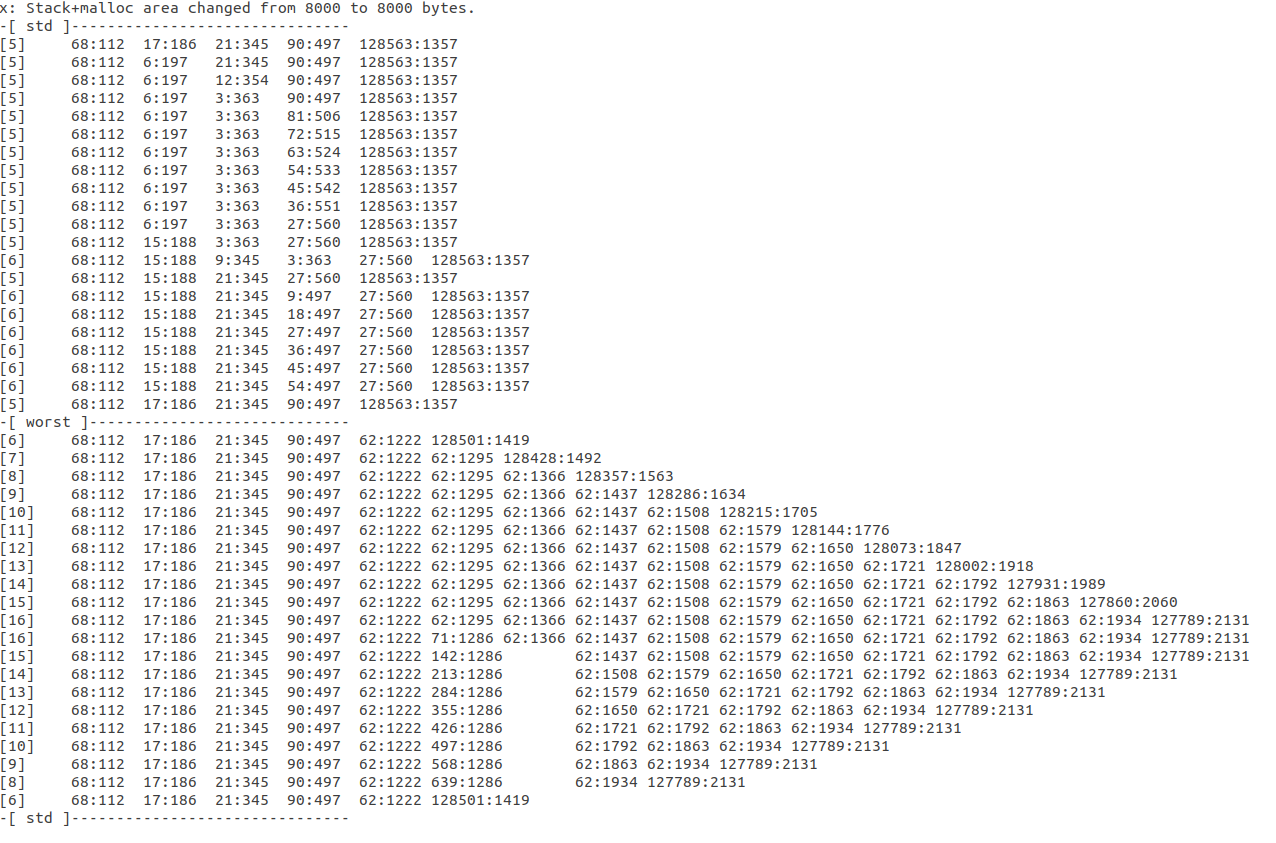
\includegraphics[width=15cm]{test.png}
    \caption{Mapy pamięci dla algorytmów \texttt{FIRST\_{}FIT} i \texttt{WORST\_{}FIT}}
	\label{fig:21}
\end{figure}



\end{document}